\documentclass[12pt]{article}

% Modelo: Mestrado/Meio ambiente/Ensaio 2/Ensaio-2_Gabriel_Cintra.tex.
% Compilar nesta pasta: latexmk -pdf analise_exploratoria.tex
\usepackage[T1]{fontenc}
\usepackage[utf8]{inputenc}
\usepackage[brazilian]{babel}
\usepackage{microtype}
\usepackage{geometry}
\geometry{a4paper, margin=2.5cm}
\usepackage{parskip}
\usepackage{amsmath,amssymb}
\usepackage{graphicx,booktabs,tabularx,array}
\usepackage{caption}
\usepackage{hyperref}
\hypersetup{colorlinks=true,urlcolor=blue,linkcolor=blue,citecolor=blue,
  pdftitle={Análise exploratória com base em Sanguinet e Azzoni (2024) e Marques et al. (2012)},
  pdfauthor={Gabriel Pincelli Cintra}}
\captionsetup{font=small,labelfont=bf,hypcap=false}
\newcolumntype{Y}{>{\raggedright\arraybackslash}X}
\setlength{\emergencystretch}{2em}
\newcommand{\instituicao}{UNIVERSIDADE FEDERAL DE SANTA CATARINA}
\newcommand{\departamento}{Programa de Pós-Graduação em Economia}
\newcommand{\curso}{Mestrado}
\newcommand{\disciplina}{Modelos de Equilíbrio Geral Computável}
\newcommand{\titulo}{Análise exploratória com base em Sanguinet e Azzoni (2024) e Marques et al. (2012)}
\newcommand{\subtitulo}{Emissões de CO\textsubscript{2} nas cadeias produtivas brasileiras}
\newcommand{\autor}{Gabriel Pincelli Cintra}
\newcommand{\local}{Florianópolis}
\newcommand{\dataentrega}{\today}
\newcommand{\imprimirtitulodois}{
\begin{center}
  {\Large\bfseries\MakeUppercase{\instituicao}\par}
  \vspace{0.2em}
  {\large \departamento\par}
  \vspace{0.2em}
  {\normalsize\textbf{\disciplina}\ (\curso)\par}
  \vspace{1.4em}
  {\LARGE\bfseries \titulo\par}
  \vspace{0.25em}
  {\large\itshape \subtitulo\par}
  \vspace{1.5em}
\end{center}
\noindent\begin{minipage}{0.48\textwidth}
  \raggedright\normalsize \autor
\end{minipage}\hfill
\begin{minipage}{0.48\textwidth}
  \raggedleft\normalsize \local, \dataentrega
\end{minipage}
\vspace{1.0em}\hrule\vspace{1.0em}
}

% SVGs completos estão em figuras/. PDFs irmãos preservam os mesmos vetores.
\newcommand{\figuraInteira}[2]{%
  \newgeometry{margin=1.2cm}
  \begin{center}
    \includegraphics[width=\linewidth,height=.91\textheight,keepaspectratio]{#1}
    \captionof{figure}{#2}
  \end{center}
  \restoregeometry
}

% Valores calculados pelo notebook; gerado por gerar_material.py.
\newcommand{\TotalBrasil}{683\,696{,}04}
\newcommand{\TotalSC}{31\,241{,}41}
\newcommand{\ParcelaSC}{4{,}57}
\newcommand{\MaiorEmissao}{56\,620{,}65}
\newcommand{\MaiorAtividade}{Eletricidade, gás e utilidades}
\newcommand{\LinhasVAB}{0191 & $309\,301{,}00$ & $146\,174{,}00$ & $163\,127{,}00$ \\
0192 & $137\,018{,}00$ & $65\,569{,}00$ & $71\,449{,}00$ \\
0280 & $32\,411{,}00$ & $8\,020{,}00$ & $24\,391{,}00$ \\
0580 & $19\,733{,}00$ & $10\,878{,}00$ & $8\,855{,}00$ \\}

\begin{document}
\imprimirtitulodois

Esse documento apresenta uma síntese da análise exploratória desenvolvida \href{https://github.com/G-Cintra/Redes/blob/main/analise_exploratoria.ipynb}{\texttt{neste notebook}} e apresentada em sala de aula.

\section*{1. Tema e objetivos}
O trabalho trata da atribuição de emissões de CO\textsubscript{2} às atividades econômicas e de sua relação com as cadeias produtivas. O local em que se emite pode diferir do local de consumo e daquele em que se obtém renda com a produção.

\textbf{Marques et al. (2012)} procuram esclarecer a responsabilidade baseada na renda e compará-la às responsabilidades pela produção e pelo consumo. \textbf{Sanguinet e Azzoni (2024)} investigam os fatores que explicam a mudança das emissões brasileiras entre 2011 e 2018, pelas perspectivas do consumo e do valor adicionado, considerando os vínculos entre estados.

\begin{center}
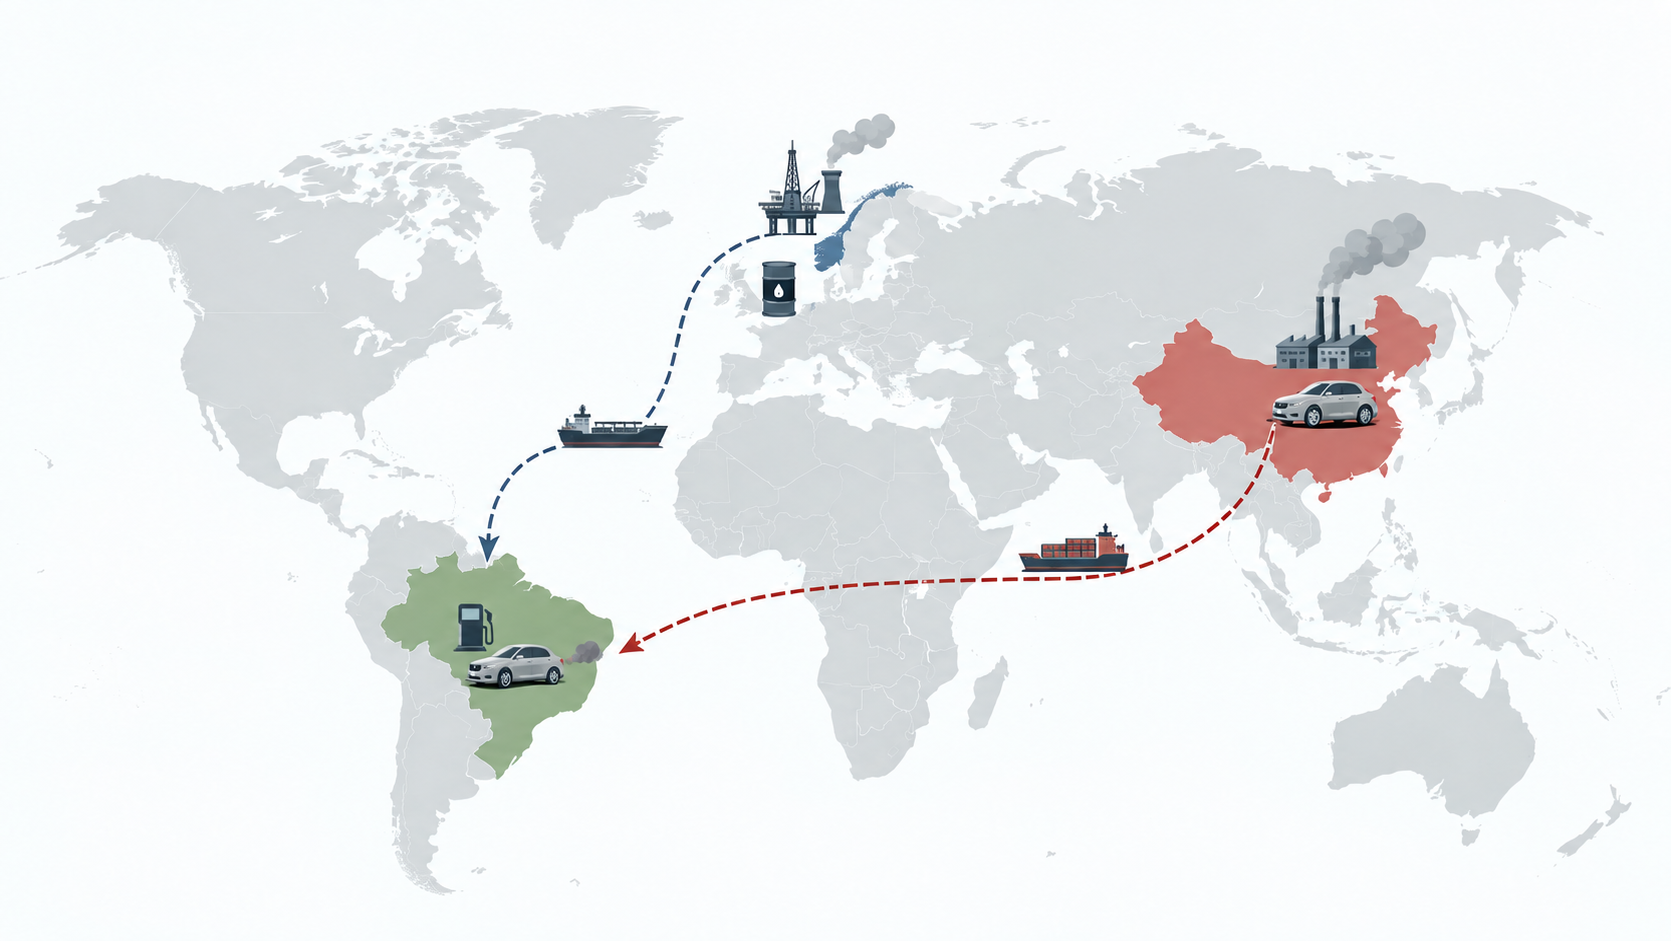
\includegraphics[width=.68\linewidth]{motivação.png}
\captionof{figure}{Motivação: produção, consumo e geração de renda podem ocorrer em países diferentes. Ilustração esquemática da apresentação, sem representar fluxos medidos.}
\end{center}

O objetivo deste exercício é calcular emissões por atividade com a MIP brasileira de 2015, verificar sua recuperação pela demanda final e explorar uma distribuição para Santa Catarina.

\newpage
\section*{2. Metodologia, dados e resultados dos artigos}
\textbf{Marques et al. (2012).} Os autores constroem um modelo multirregional mundial com a base GTAP 7.1, para 2004, abrangendo 112 países ou regiões. Combinam transações intermediárias, produção, demanda final, valor adicionado e emissões. A inversa de Leontief atribui emissões à demanda final; a inversa de Ghosh permite a atribuição aos fornecedores de fatores primários, pela renda. A produção corresponde às emissões diretas territoriais.

\textbf{Sanguinet e Azzoni (2024).} Utilizam matrizes inter-regionais do NEREUS-USP, com 27 UFs e 67 setores, para 2011 e 2018. Atualizam fluxos com Contas Regionais do IBGE e balanceamento RAS; os valores de 2011 são ajustados pelo IPCA para dezembro de 2018. Compatibilizam emissões EORA/EDGAR com os setores da MIP e adotam intensidade nacional uniforme por setor entre as UFs. A decomposição estrutural identifica contribuições da intensidade, da estrutura produtiva, da demanda e dos fatores associados ao valor adicionado.

\begin{center}
\small
\begin{tabularx}{\linewidth}{Y l r r}
\toprule
Referência e recorte & Critério & Primeiro ano & Segundo ano\\
\midrule
Marques: Brasil, Mt de CO$_2$ & Produção & 234,81 (2004) & ---\\
 & Consumo & 215,53 (2004) & ---\\
 & Renda & 241,66 (2004) & ---\\
\midrule
Sanguinet--Azzoni: Brasil, & Demanda & 589.974 (2011) & 783.654 (2018)\\
Gg de CO$_2$ & Oferta/renda & 503.523 (2011) & 639.057 (2018)\\
\bottomrule
\end{tabularx}
\captionof{table}{Resultados publicados: Marques et al., Tabela 2, p.~61; Sanguinet e Azzoni, Tabela 3, p.~7. As contas diferem em ano, unidade e recorte; 1 Mt = 1.000 Gg.}
\end{center}

Para Marques et al., os critérios redistribuem a responsabilidade sem modificar o total mundial. O caso da Noruega evidencia emissões habilitadas no exterior pela exportação de combustíveis, pouco visíveis nas contas de produção e consumo. As diferenças são especialmente relevantes em economias pequenas e abertas.

Sanguinet e Azzoni destacam a distribuição desigual dos benefícios econômicos e das emissões entre regiões. Pela demanda, sobressaem estrutura produtiva, exportações e demanda doméstica; pela renda, estrutura de alocação e atividade econômica. Regiões mais ricas podem beneficiar-se de insumos intensivos em emissões provenientes de regiões menos desenvolvidas.



\newpage
\section*{3. Dados e hipóteses do exercício}
Neste exercício, atribuímos as emissões às atividades produtoras: $c_i$ identifica quem emite. O cálculo $\Phi Ly$ mantém essa atribuição, embora utilize a demanda final. A atribuição ao setor de demanda final seria $\operatorname{diag}(y)L^{\mathsf T}\varphi$. A conta de renda/Ghosh não é estimada; a igualdade analisada adiante refere-se às emissões por atividade produtora.

Usamos vetores coluna em minúsculas e matrizes em maiúsculas. Os códigos identificam as atividades da MIP do IBGE.

\begin{center}
\small\renewcommand{\arraystretch}{1.22}
\begin{tabularx}{\linewidth}{l l Y l}
\toprule
Objeto & Dimensão & Significado e unidade & Fonte na MIP\\
\midrule
$x$ & $67\times1$ & Produção; R\$ milhões & 01!H134:BV134\\
$L$ & $67\times67$ & Inversa de Leontief; adimensional & 15!C6:BQ72\\
$f$ & $127\times1$ & Demanda final nacional por produto, com exportações; R\$ milhões & 03!BZ6:BZ132\\
$D$ & $67\times127$ & Participação das atividades na produção dos produtos; adimensional & 13!C6:DY72\\
$y=Df$ & $67\times1$ & Demanda final por atividade; R\$ milhões & Conversão por $D$\\
$\varphi$ & $67\times1$ & Intensidades; Gg CO$_2$/R\$ milhão & Artigo, Tabela 2\\
$\Phi$ & $67\times67$ & Intensidades na diagonal & $\operatorname{diag}(\varphi)$\\
$ci$ & $67\times1$ & Consumo intermediário; R\$ milhões & 02!C134:BQ134\\
\bottomrule
\end{tabularx}
\captionof{table}{Entradas utilizadas. Os números 01, 02, 03, 13 e 15 identificam as abas da MIP de 2015, nível 67.}
\end{center}

\textbf{Hipóteses e recorte da análise}
\begin{itemize}
\item \textbf{Estrutura econômica:} usamos a MIP nacional do IBGE de \textbf{2015}, com 67 atividades e 127 produtos. As emissões são atribuídas às atividades produtoras, incluindo a produção para exportação e excluindo emissões ocorridas no exterior associadas às importações.
\item \textbf{Coeficientes de emissão:} aproximamos as intensidades de 2015 por interpolação linear dos coeficientes de 2011 e 2018 de Sanguinet e Azzoni: $\varphi_{2015}=\varphi_{2011}+\frac{4}{7}(\varphi_{2018}-\varphi_{2011})$. Assumimos variação linear no período e aplicamos os coeficientes à produção de 2015 sem ajuste adicional de preços. As emissões resultantes são estimativas do cenário, não um inventário observado de 2015.
\item \textbf{Estimativa para SC:} distribuímos uma parcela da produção brasileira entre as 20 microrregiões históricas por pesos baseados no VAB de 2015 e em hipóteses de especialização setorial, apoiadas em fontes de diferentes anos. Mantemos a intensidade nacional de cada atividade em todas as regiões e preservamos sua participação estadual estimada pela base do VAB.
\item \textbf{Comparação com o satélite:} comparamos as emissões estimadas de \textbf{CO$_2$, com base econômica em 2015}, à coluna troposférica de \textbf{NO$_2$ observada em 2023} pelo Sentinel-5P/TROPOMI. A comparação descreve padrões espaciais de gases, grandezas e anos diferentes; não constitui validação direta das emissões estimadas.
\end{itemize}

\newpage
\section*{4. Cálculo das emissões pela produção e pela demanda}
A demanda final da MIP é apresentada por produto. Para relacioná-la às atividades produtoras, utilizamos a matriz de participação $D$, obtendo $y=Df$. A inversa de Leontief relaciona essa demanda à produção necessária em toda a cadeia: $x=Ly$.

Cada atividade possui uma intensidade de emissão $\varphi_i$, que expressa quanto CO$_2$ é emitido por unidade monetária produzida. Reunindo essas intensidades na diagonal de $\Phi$, calculamos:
\[
c=\Phi x.
\]
O elemento $c_i=\varphi_i x_i$ representa as emissões da atividade $i$ associadas à sua produção, destinada tanto a usos intermediários quanto à demanda final doméstica e às exportações.

Substituindo a produção por sua relação com a demanda final, temos:
\[
c=\Phi Ly=Cy,\qquad C=\Phi L.
\]
Multiplicar $\Phi$ por $L$  equivale a ponderar cada linha da inversa de Leontief pela intensidade da atividade emissora. Em seguida, multiplicar $C$ por $y$ pondera cada coluna pela demanda final correspondente. Para cada atividade, o resultado é:
\[
c_i=\sum_j C_{ij}y_j=\varphi_i\sum_jL_{ij}y_j.
\]
As duas expressões recuperam as mesmas emissões no sistema completo. A primeira utiliza diretamente a produção observada; a segunda explica essa produção pela demanda final e pelos encadeamentos produtivos. Em ambas, a atribuição permanece na atividade que emite.

\section*{5. Interpretação da matriz de emissões}
A matriz $C$ permite examinar os encadeamentos antes de ponderá-los pela demanda observada. Cada elemento $C_{ij}=\varphi_iL_{ij}$ mede as emissões na atividade $i$ necessárias para atender a uma unidade monetária de demanda final da atividade $j$. As linhas identificam quem emite e as colunas identificam a atividade que recebe a demanda final.

Na diagonal, $C_{ii}$ inclui a produção final e os retornos da cadeia à própria atividade; portanto, seu significado é mais amplo que o da intensidade direta $\varphi_i$. A soma de uma coluna reúne as emissões de todas as atividades necessárias para atender à demanda unitária de $j$.

O heatmap abaixo apresenta a matriz completa. A escala logarítmica permite visualizar coeficientes de ordens de grandeza distintas: tons claros representam valores menores e tons escuros, maiores. Os zeros são exibidos na cor mais clara e não entram na transformação logarítmica.

\figuraInteira{figuras/heatmap_c.pdf}{Matriz completa $C=\Phi L$, com as 67 atividades nas linhas e colunas. Unidade: Gg de CO$_2$ por R\$ milhão de demanda final. Escala logarítmica; zeros na cor mais clara.}

\section*{6. Emissões e valor adicionado bruto}
O VAB permite relacionar a emissão de cada atividade à sua participação econômica. Apresentamos três indicadores na figura abaixo: emissão absoluta $c_i$; razão entre a participação nas emissões e a participação no VAB; e participação no VAB nacional:
\[
I_i=\frac{c_i/\sum_jc_j}{vab_i/\sum_jvab_j},\qquad
P_i=100\frac{vab_i}{\sum_jvab_j}.
\]
Se $I_i>1$, a atividade participa mais das emissões do que do VAB. Se $I_i<1$, ocorre o inverso. O índice é adimensional; não é a intensidade de emissões por unidade monetária.

\figuraInteira{figuras/emissoes_vab.pdf}{Emissões, razão entre participações nas emissões e no VAB, e participação no VAB: 67 atividades ordenadas da maior para a menor emissão. Todos os indicadores e atividades do notebook são apresentados.}

\section*{7. Estimativa para as microrregiões de SC}
Distribuímos uma parcela da produção brasileira entre 20 microrregiões de SC. A matriz $W$ ($67\times20$) contém a fração da produção nacional do setor $i$ atribuída à região $r$.

Os pesos partem da participação microrregional no VAB brasileiro de 2015, em quatro grupos (IBGE/SIDRA, tabela 5938), e de fatores hipotéticos de especialização setorial. Esses fatores redistribuem a produção dentro de SC, preservando a participação estadual da base VAB; não são medidas observadas de produção setorial.
\[
q_i=\sum_rW_{ir},\qquad S_{ir}=\frac{W_{ir}}{q_i},\qquad\sum_rS_{ir}=1.
\]
O vetor $q$ ($67\times1$) representa a participação estadual; $S$ ($67\times20$), a distribuição de cada setor dentro de SC.

Aplicamos os pesos à produção e mantemos a intensidade nacional por atividade:
\[
X^{SC}_{ir}=W_{ir}x_i,\quad E^{SC}_{ir}=\varphi_iX^{SC}_{ir}=W_{ir}c_i,
\quad e^{SC}_r=\sum_iE^{SC}_{ir}.
\]
$X^{SC}$ e $E^{SC}$ têm dimensão $67\times20$; somamos as atividades de cada \textbf{coluna} para obter $e^{SC}$ ($20\times1$). Assim, $e^{SC}=W^{\mathsf T}c$ e $\sum_re^{SC}_r=\sum_iq_ic_i$.

\figuraInteira{figuras/pesos_sc.pdf}{Distribuição completa dos 67 setores entre as 20 microrregiões: $100S_{ir}$. Cada linha soma 100\% antes do arredondamento. Os números representam participações na produção estadual de cada atividade.}

\section*{8. Resultados regionais e comparação espacial}


Comparamos o mapa estimado à coluna troposférica de NO$_2$ de 2023 do Sentinel-5P/TROPOMI (FMI/SAMPO). A composição anual tem grade de $0{,}05^\circ$, filtro de qualidade de origem $qa>0{,}75$ e recorte terrestre IBGE/GSHHG. Utilizamos células válidas com peso HARP positivo.
\begin{center}
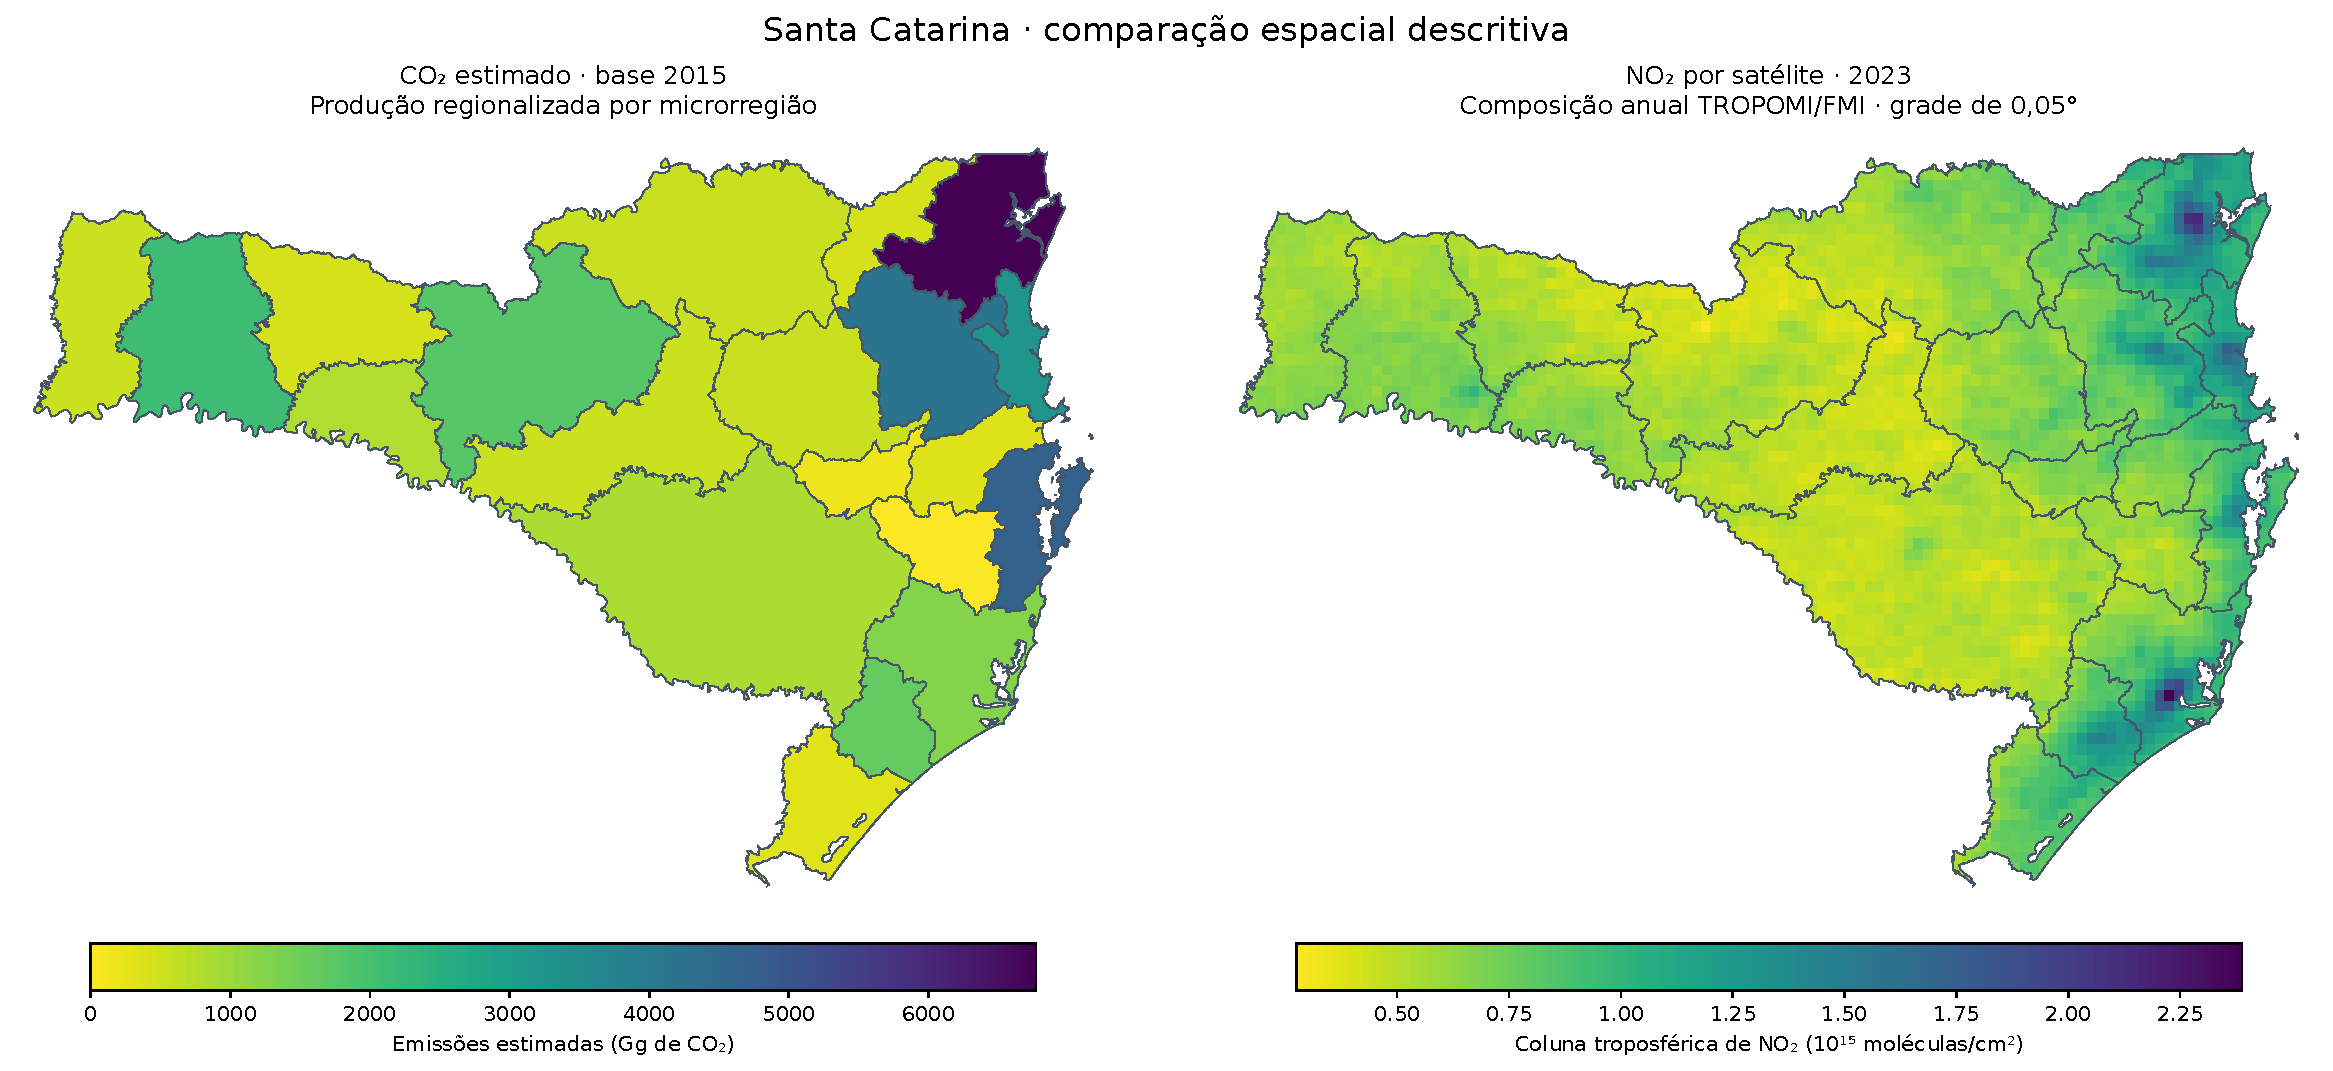
\includegraphics[width=\linewidth]{figuras/comparacao_satelite.pdf}
\captionof{figure}{Comparação completa entre os totais regionais de CO$_2$ estimados (base 2015) e a coluna de NO$_2$ observada por satélite (2023). Os painéis usam escalas próprias e preservam todas as microrregiões e células válidas do recorte.}
\end{center}

\section*{9. Conclusões}
Os artigos mostram que produção, consumo e renda permitem leituras distintas da responsabilidade ambiental. O exercício verifica uma identidade mais restrita: mantendo o setor emissor como referência, $c=\Phi x=\Phi Ly$. A matriz $C$ evidencia os encadeamentos e o VAB permite comparar participação econômica e participação nas emissões.

A estimativa para SC ilustra uma distribuição espacial condicionada ao VAB, aos pesos setoriais e à intensidade nacional uniforme. O satélite acrescenta uma comparação descritiva, mas não valida o CO$_2$ estimado: mede outro gás, outra grandeza e outro ano. Avanços exigem compatibilização monetária dos coeficientes e dados regionais de produção e tecnologia.

\paragraph*{Referências}
{\footnotesize
SANGUINET, E. R.; AZZONI, C. R. Carbon emissions drivers in Brazilian regional production chains: Value-added and consumption-based approaches. \textit{Regional Science Policy \& Practice}, v.~16, 100015, 2024. \href{https://doi.org/10.1016/j.rspp.2024.100015}{DOI: 10.1016/j.rspp.2024.100015}.

MARQUES, A.; RODRIGUES, J.; LENZEN, M.; DOMINGOS, T. Income-based environmental responsibility. \textit{Ecological Economics}, v.~84, p.~57--65, 2012. \href{https://doi.org/10.1016/j.ecolecon.2012.09.010}{DOI: 10.1016/j.ecolecon.2012.09.010}.

\textbf{Dados:} IBGE, MIP 2015 e SIDRA 5938; Copernicus/FMI, \href{https://sampo.fmi.fi/tropomi_l3/info_dev.php}{TROPOMI/SAMPO}, NO$_2$ de 2023. Arquivos e hipóteses identificados no notebook.\par}
\end{document}
